\subsection{Concurrency in Device Drivers}
\label{bg:concurrency}

Nowadays, multicore machines have become mainstream, allowing operating systems to exploit concurrency for \emph{responsiveness} (latency) or \emph{performance} (throughput). In drivers, responsiveness is important (even if there is only a single core available), because entry points of distinct processes should run concurrently so that no single process hogs the core. Likewise, performance is important, as drivers should be able to timely process incoming requests (e.g.\ network packages).

Modern operating systems address the demand for responsiveness and performance by providing multiple sources of concurrency~\cite{corbet2005linux}: a kernel can invoke an arbitrary number of entry points from the same driver concurrently; a running driver process can block and be replaced by another process in the same driver; hardware interrupts can be handled concurrently; delayed code execution is the norm; and the user can insert or remove hardware components without rebooting the kernel (known as hot-plugging). All these possibilities can easily lead to \emph{data races}, which can be defined as follows:

\begin{definition}
\label{definition:datarace}
A data race occurs when two distinct threads access a shared memory location, at least one of the accesses modifies the location, at least one of the accesses is non-atomic, and there is no mechanism in place to prevent these accesses from being simultaneous.
\end{definition}

Example~\ref{fig:data_race_example} presents multiple data races that \whoop automatically found in the generic\_nvram Linux char driver (see Section~\ref{evaluation}). The driver can invoke the \texttt{nvram\_llseek} entry point concurrently from two threads $T_1$ and $T_2$, while passing the same \texttt{file} object as a parameter. However, this can lead to multiple possible data races, because $T_1$ and $T_2$ can read/write access the \texttt{f\_pos} field of the \texttt{file} object in arbitrary order resulting into nondeterministic behavior.

\begin{figure}[t]
\begin{lstlisting}
static loff_t nvram_llseek(struct file *file,
    loff_t offset, int origin) {
  switch (origin) {
    case 0: break;
    case 1: offset += file->f_pos; break; // racy
    case 2: offset += nvram_len; break;
    default: offset = -1;
  }
  if (offset < 0)
    return -EINVAL;
  file->f_pos = offset; // racy
  return file->f_pos; // racy
}
\end{lstlisting}
\caption{Example of data races in the generic\_nvram Linux char driver}
\label{fig:data_race_example}
\end{figure}

The most common technique for eliminating data races is using a \emph{locking} mechanism. Locking a set of program statements that access a shared resource creates a \emph{critical section}, i.e.\ source code that cannot be executed by more than one thread simultaneously. Figure~\ref{fig:lock_example} shows how to use a lock to eliminate the data race in Figure~\ref{fig:data_race_example}. The example is tricky, because the return statement can potentially race on the \texttt{f\_pos} field. To fix this issue, we store the result in a temporary variable, inside the critical section.

Lock-based synchronization is a powerful tool for preventing data races in drivers, but careless use of locks has multiple pitfalls~\cite{sutter2005software}. Coarse-grained locking can hurt performance, because it limits the opportunity for concurrency. On the other hand, fine-grained locking can easily lead to deadlocks. Although the Linux kernel provides sophisticated lock-free synchronization mechanisms~\cite{corbet2005linux}, such as atomic read and write operations, in this work we focus on locks. However, we still treat lock-free operations (e.g.\ atomics) soundly (see Definition~\ref{definition:datarace}), by not regarding them as providing any protection between threads. This is sound but can potentially introduce false positives.

We believe that our focus in locks is justified, because the majority of Linux drivers still use locks. To check this, we used a simple grep command and found that 68\% of the drivers from the 4.0 Linux kernel distribution use locks, versus 13\% that use atomic operations. We also found that 31\% of the drivers use neither locking nor atomic primitives, which suggests that they are either simple (non-concurrent) drivers or use some other lock-free synchronization primitive.

\begin{figure}[t]
\begin{lstlisting}
static loff_t nvram_llseek(struct file *file,
    loff_t offset, int origin) {
  mutex_lock(&nvram_mutex); // lock
  switch (origin) {
    case 0: break;
    case 1: offset += file->f_pos; break;
    case 2: offset += nvram_len; break;
    default: offset = -1;
  }
  if (offset < 0)
    return -EINVAL;
  file->f_pos = offset;
  loff_t res = file->f_pos; // store result
  mutex_unlock(&nvram_mutex); // unlock
  return res;
}
\end{lstlisting}
\caption{Using a lock to eliminate the data races in the previous example}
\label{fig:lock_example}
\end{figure}

\subsection{Lockset Analysis}
\label{bg:lockset}

Lockset analysis is a lightweight race detection method proposed in the context of Eraser~\cite{savage1997eraser}, a dynamic data race detector.  The idea is to track the set of locks that are \emph{consistently} used to protect a memory location during program execution. If that lockset ever becomes empty, the analysis reports a potential data race on that memory location. This is because an inconsistent lockset suggests that a memory location \emph{may} be accessed simultaneously by two or more threads.  

\begin{figure}[htbp]
\centering
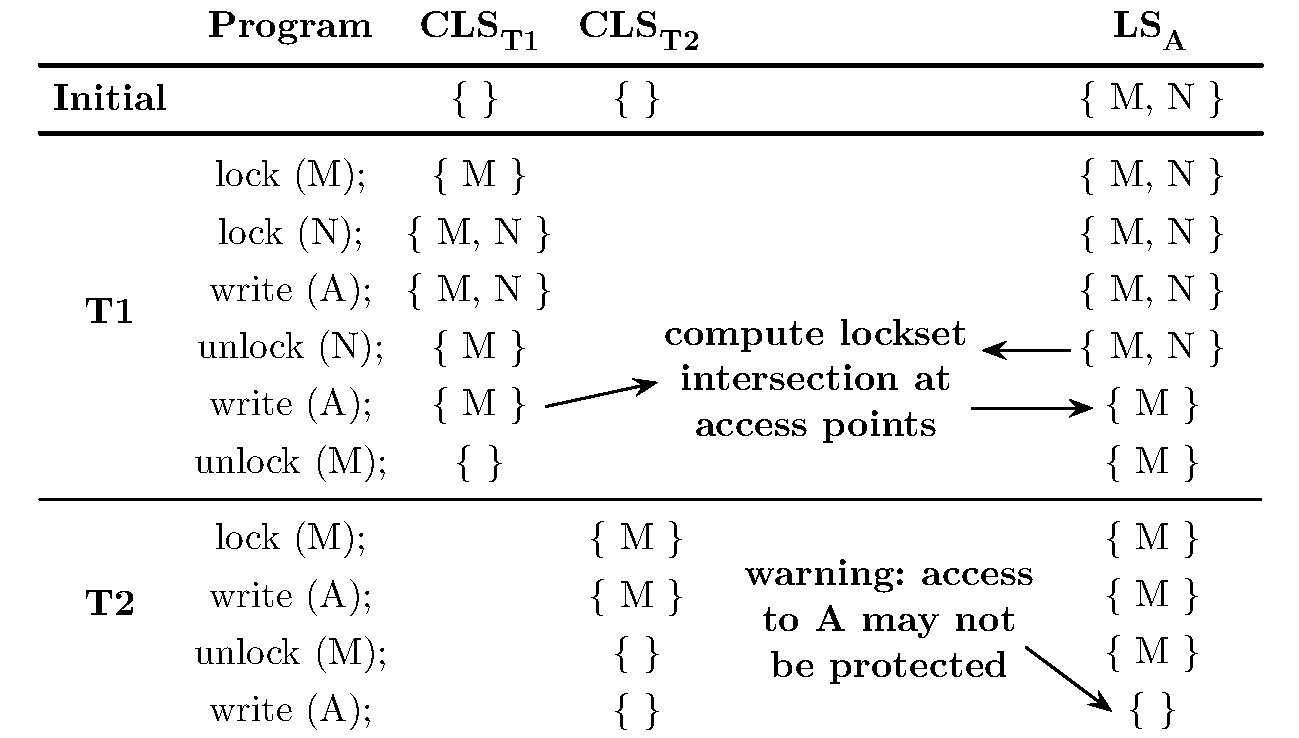
\includegraphics[width=1\linewidth]{img/lockset.pdf}
\caption{Applying lockset analysis on a thread of a concurrent program}
\label{fig:locksets}
\end{figure}

Lockset analysis for a concurrent program starts by creating a \emph{current} lockset, $\mathit{CLS}_T$, for each thread $T$ of the program, and a lockset, $\mathit{LS}_v$, for each shared variable $v$ used in the program. Initially, $\mathit{CLS}_T$ is empty for every thread $T$, because the threads do not hold any locks on program start. The lockset $\mathit{LS}_v$ for each variable $v$ is initialized to the set of all locks manipulated by the program, because initially each access to $v$ has (vacuously) been protected by every lock. The program is executed as usual (with threads scheduled according to the OS scheduler), except that instrumentation is added to update locksets as follows:
%
\begin{enumerate}
\item After each \emph{lock} and \emph{unlock} operation by $T$, $\mathit{CLS}_T$ is updated to reflect the locks currently held by $T$.
\item When $T$ accesses shared variable $v$, any locks that are not common to $\mathit{LS}_v$ and $\mathit{CLS}_T$ are removed from $\mathit{LS}_v$.
If $\mathit{LS}_v$ becomes empty as a result, a warning is issued that the access to $v$ may be unprotected.
\end{enumerate}

Figure~\ref{fig:locksets} shows an example of applying lockset analysis on a concurrent program consisting of two threads $T_1$ and $T_2$, both accessing a global variable $A$. Initially, $\mathit{LS}_A$, which is the lockset for A, contains all possible locks in the program: $M$ and $N$. During execution of $T_1$, the thread writes $A$ without holding $N$, and thus $N$ is removed from $\mathit{LS}_A$. Next, during execution of $T_2$, the thread writes $A$ without holding $M$, and thus $\mathit{LS}_A$ becomes empty. Finally, a warning is reported because the two threads do not consistently protect $A$.

In contrast to more sophisticated race analyses that encode a \emph{happens-before} relation between threads~\cite{lamport1978time} (e.g.\ using vector clocks), lockset analysis is easy to implement, lightweight, and thus has the potential to scale well.  The technique, though, suffers from imprecision (i.e.\ can report false bugs), because a violation of the locking discipline does not always correspond to a real data race~\cite{savage1997eraser, pozniansky2003efficient, o2003hybrid, elmas2007goldilocks, flanagan2009fasttrack}. Furthermore, the code coverage in dynamic lockset analyzers, such as Eraser, is limited by the execution paths that are explored under a given scheduler. This is because the tool runs the program in a truly concurrent environment, thus it only gets to see what the thread did on the particular schedule that was followed.

To counter the above limitations, techniques such as Locksmith~\cite{pratikakis2006locksmith} and RELAY~\cite{voung2007relay} have explored the idea of applying lockset analysis in a static context, using dataflow analysis. In this paper, we present a novel symbolic lockset analysis method that involves generating verification conditions, which are then discharged to a theorem prover.
